% Template for ICIP-2019 paper; to be used with:
%          spconf.sty  - ICASSP/ICIP LaTeX style file, and
%          IEEEbib.bst - IEEE bibliography style file.
% --------------------------------------------------------------------------
%https://www.overleaf.com/9666543272fnzcnqpkqjxp

\documentclass{article}
\usepackage{spconf}
\usepackage[utf8]{inputenc}

\usepackage{amsmath}
\usepackage{amssymb}
\usepackage{amsfonts}
\usepackage{multirow}
\usepackage{multicol}
\usepackage{graphicx}
\usepackage{float}
\usepackage{caption}
\usepackage[font=footnotesize]{subcaption}
\usepackage{array}
\usepackage{color}
\usepackage{colortbl}
\usepackage[table]{xcolor}
\usepackage{ntheorem}
\usepackage{IEEEtrantools}
\usepackage[color=blue!20]{todonotes}
\usepackage{hyperref}
\usepackage{url}
%\usepackage{subfigure}
\usepackage{booktabs}
\usepackage{tikz}
\usepackage{flushend}

% My Table

\colorlet{tableheadcolor}{gray!25} % Table header colour = 25% gray
\colorlet{tablerowcolor}{gray!10} % Table row separator colour = 10% gray

\newcommand{\headcol}{\rowcolor{tableheadcolor}} %
\newcommand{\rowcol}{\rowcolor{tablerowcolor}} %

% Command \topline consists of a (slightly modified) \toprule followed by a \heavyrule rule of colour tableheadcolor (hence, 2 separate rules)
\newcommand{\topline}{\arrayrulecolor{black}\specialrule{0.1em}{\abovetopsep}{0pt}%
    \arrayrulecolor{tableheadcolor}\specialrule{\belowrulesep}{0pt}{0pt}%
    \arrayrulecolor{black}}

% Command \midline consists of 3 rules (top colour tableheadcolor, middle colour black, bottom colour white)
\newcommand{\midline}{\arrayrulecolor{tableheadcolor}\specialrule{\aboverulesep}{0pt}{0pt}%
    \arrayrulecolor{black}\specialrule{\lightrulewidth}{0pt}{0pt}%
    \arrayrulecolor{white}\specialrule{\belowrulesep}{0pt}{0pt}%
    \arrayrulecolor{black}\hline}

% Command \rowmidlinecw consists of 3 rules (top colour tablerowcolor, middle colour black, bottom colour white)
\newcommand{\rowmidlinecw}{\arrayrulecolor{tablerowcolor}\specialrule{\aboverulesep}{0pt}{0pt}%
    \arrayrulecolor{black}\specialrule{\lightrulewidth}{0pt}{0pt}%
    \arrayrulecolor{white}\specialrule{\belowrulesep}{0pt}{0pt}%
    \arrayrulecolor{black}}

% Command \rowmidlinewc consists of 3 rules (top colour white, middle colour black, bottom colour tablerowcolor)
\newcommand{\rowmidlinewc}{\arrayrulecolor{white}\specialrule{\aboverulesep}{0pt}{0pt}%
    \arrayrulecolor{black}\specialrule{\lightrulewidth}{0pt}{0pt}%
    \arrayrulecolor{tablerowcolor}\specialrule{\belowrulesep}{0pt}{0pt}%
    \arrayrulecolor{black}}

% Command \rowmidlinew consists of 1 white rule
\newcommand{\rowmidlinew}{\arrayrulecolor{white}\specialrule{\aboverulesep}{0pt}{0pt}%
    \arrayrulecolor{black}}

% Command \rowmidlinec consists of 1 tablerowcolor rule
\newcommand{\rowmidlinec}{\arrayrulecolor{tablerowcolor}\specialrule{\aboverulesep}{0pt}{0pt}%
    \arrayrulecolor{black}}

% Command \bottomline consists of 2 rules (top colour
\newcommand{\bottomline}{\arrayrulecolor{white}\specialrule{\aboverulesep}{0pt}{0pt}%
    \arrayrulecolor{black}\specialrule{\heavyrulewidth}{0pt}{\belowbottomsep}}%
\newcommand{\bottomlinec}{\arrayrulecolor{tablerowcolor}\specialrule{\aboverulesep}{0pt}{0pt}%
    \arrayrulecolor{black}\specialrule{\heavyrulewidth}{0pt}{\belowbottomsep}}%
\newcommand{\bottomlinehc}{\arrayrulecolor{tableheadcolor}\specialrule{\aboverulesep}{0pt}{0pt}%
    \arrayrulecolor{black}\specialrule{\heavyrulewidth}{0pt}{\belowbottomsep}}%

\newcommand*{\rulefillerh}{%
    \arrayrulecolor{tableheadcolor}% change to cell colour
    \specialrule{\heavyrulewidth}{0pt}{-\heavyrulewidth}% "invisible" rule
    \arrayrulecolor{black}% revert to regular line colour
}

\newcommand*{\rulefillerc}{%
    \arrayrulecolor{tablerowcolor}% change to cell colour
    \specialrule{\heavyrulewidth}{0pt}{-\heavyrulewidth}% "invisible" rule
    \arrayrulecolor{black}% revert to regular line colour
}

\let\mcol\multicolumn
\let\ml\multirow



% Example definitions.
% --------------------
\def\x{{\mathbf x}}
\def\L{{\cal L}}
\newcommand{\etal}[1]{#1~\textit{et~al.}}
%% My Table

\colorlet{tableheadcolor}{gray!25} % Table header colour = 25% gray
\colorlet{tablerowcolor}{gray!10} % Table row separator colour = 10% gray

\newcommand{\headcol}{\rowcolor{tableheadcolor}} %
\newcommand{\rowcol}{\rowcolor{tablerowcolor}} %

% Command \topline consists of a (slightly modified) \toprule followed by a \heavyrule rule of colour tableheadcolor (hence, 2 separate rules)
\newcommand{\topline}{\arrayrulecolor{black}\specialrule{0.1em}{\abovetopsep}{0pt}%
    \arrayrulecolor{tableheadcolor}\specialrule{\belowrulesep}{0pt}{0pt}%
    \arrayrulecolor{black}}

% Command \midline consists of 3 rules (top colour tableheadcolor, middle colour black, bottom colour white)
\newcommand{\midline}{\arrayrulecolor{tableheadcolor}\specialrule{\aboverulesep}{0pt}{0pt}%
    \arrayrulecolor{black}\specialrule{\lightrulewidth}{0pt}{0pt}%
    \arrayrulecolor{white}\specialrule{\belowrulesep}{0pt}{0pt}%
    \arrayrulecolor{black}\hline}

% Command \rowmidlinecw consists of 3 rules (top colour tablerowcolor, middle colour black, bottom colour white)
\newcommand{\rowmidlinecw}{\arrayrulecolor{tablerowcolor}\specialrule{\aboverulesep}{0pt}{0pt}%
    \arrayrulecolor{black}\specialrule{\lightrulewidth}{0pt}{0pt}%
    \arrayrulecolor{white}\specialrule{\belowrulesep}{0pt}{0pt}%
    \arrayrulecolor{black}}

% Command \rowmidlinewc consists of 3 rules (top colour white, middle colour black, bottom colour tablerowcolor)
\newcommand{\rowmidlinewc}{\arrayrulecolor{white}\specialrule{\aboverulesep}{0pt}{0pt}%
    \arrayrulecolor{black}\specialrule{\lightrulewidth}{0pt}{0pt}%
    \arrayrulecolor{tablerowcolor}\specialrule{\belowrulesep}{0pt}{0pt}%
    \arrayrulecolor{black}}

% Command \rowmidlinew consists of 1 white rule
\newcommand{\rowmidlinew}{\arrayrulecolor{white}\specialrule{\aboverulesep}{0pt}{0pt}%
    \arrayrulecolor{black}}

% Command \rowmidlinec consists of 1 tablerowcolor rule
\newcommand{\rowmidlinec}{\arrayrulecolor{tablerowcolor}\specialrule{\aboverulesep}{0pt}{0pt}%
    \arrayrulecolor{black}}

% Command \bottomline consists of 2 rules (top colour
\newcommand{\bottomline}{\arrayrulecolor{white}\specialrule{\aboverulesep}{0pt}{0pt}%
    \arrayrulecolor{black}\specialrule{\heavyrulewidth}{0pt}{\belowbottomsep}}%
\newcommand{\bottomlinec}{\arrayrulecolor{tablerowcolor}\specialrule{\aboverulesep}{0pt}{0pt}%
    \arrayrulecolor{black}\specialrule{\heavyrulewidth}{0pt}{\belowbottomsep}}%
\newcommand{\bottomlinehc}{\arrayrulecolor{tableheadcolor}\specialrule{\aboverulesep}{0pt}{0pt}%
    \arrayrulecolor{black}\specialrule{\heavyrulewidth}{0pt}{\belowbottomsep}}%

\newcommand*{\rulefillerh}{%
    \arrayrulecolor{tableheadcolor}% change to cell colour
    \specialrule{\heavyrulewidth}{0pt}{-\heavyrulewidth}% "invisible" rule
    \arrayrulecolor{black}% revert to regular line colour
}

\newcommand*{\rulefillerc}{%
    \arrayrulecolor{tablerowcolor}% change to cell colour
    \specialrule{\heavyrulewidth}{0pt}{-\heavyrulewidth}% "invisible" rule
    \arrayrulecolor{black}% revert to regular line colour
}

\let\mcol\multicolumn
\let\ml\multirow


\newcommand{\dataset}{{\cal D}}
\newcommand{\fracpartial}[2]{\frac{\partial #1}{\partial  #2}}
\newcommand{\highlight}[1]{\tikz[baseline]{\node[rounded corners,fill=green!25, anchor=base]{$\mathbf{#1}$}}}

% Title.
% ------
\title{Scene Text Detection Using Mobile Object Detection Network}
%
% Single address.
% ---------------
\name{\parbox{0.99\linewidth}{\centering{%
Luis Decker$^1$,
Allan~Pinto$^1$,
Jose Luis Flores Campana$^1$,
Manuel C\'{o}rdova Neira$^1$,
Andreza A. dos Santos,$^1$,
Jhonatas S. Concei\c{c}\~{a}o$^1$,
Marcus A. Angeloni$^2$,
Lin Tzy Li$^2$,
and Ricardo da S. Torres$^1$}~\thanks{We thank Samsung R\&D Institute Brazil and CNPq for the financial support. Authors are also grateful to  S\~ao Paulo Research Foundation -- FAPESP (grants \#2014/12236-1, \#2015/24494-8, \#2016/50250-1, and \#2017/20945-0).
This study was financed in part by the Coordena\c c\~ao de Aperfei\c coamento de Pessoal de N\'ivel Superior - Brasil (CAPES) - Finance Code 001.}
}}
\address{$^1$RECOD Lab., Institute of Computing, University of Campinas, 13083-852, Brazil\\
$^2$AI R\&D, Samsung R\&D Institute Brazil, 13097-160, Brazil 
}

\begin{document}
\ninept
%\setlength{\belowcaptionskip}{-10pt}

\tolerance=999 %[marcus] para evitar que o texto extrapole a largura das colunas

%
\maketitle
%
Multiple research initiatives have been reported to yield highly effective results for the text detection problem, which consists of the challenge of detecting in a digital image if there is a textual element, like a word or a phrase. However, most of those solutions are very costly, thus hampering their use in several applications that rely on the use of devices with restricted processing power, like smartwatches and mobile phones. The text localization is an important step on very widely-used  applications that can be executed on mobile environments, like on-the-go translations and recognition of text for the visually impaired. In this work, we address this issue by investigating the use of efficient object detection networks for this problem. We propose the combination of two light architectures, MobileNetV2 and Single Shot Detector~(SSD), into our proposal MobText for the text detection problem. %Experimental results on the ICDAR'11 and ICDAR'13 datasets demonstrate that our solution yields comparable or superior effectiveness performance than several baselines of the literature, with a low processing cost.
Experimental results in the ICDAR'11 and ICDAR'13 datasets demonstrate that our solution yields the best trade-off between effectiveness and efficiency in terms of processing time, and also achieved the state-of-the-art results in the ICDAR'11 dataset with an f-measure of $96.09\%$ and an average processing time of $464 ms$ on a restricted processing device.  Another contribution of this work relies on the proposal of an evaluation tool to support the assessment of text localization and recognition methods.
%\section{Introduction}
\label{sec:introduction}

Reading text in images is still an open problem in computer vision and image understanding research fields. This problem has attracted a lot of attention to these communities due to a large number of modern applications that can potentially benefit from this knowledge, such as self-driving vehicles~\cite{Yan2018TITS,Zhu2018TITS}, robot navigation, scene understanding~\cite{Wang2018IJCV}, assistive technologies~\cite{Yi2014TM}, among others. In addition, the ubiquity of mobile and wearable devices led the text detection and recognition problems to a high-order complexity in terms of efficiency and effectiveness, as both are expected to be performed in real-time in several practical usage scenarios. Thereby, the conception of methods for understanding texts in images effectively and at low computation costs is of paramount importance.

Several methods have been recently proposed in the literature towards localizing textual information in scene images. In general, the text reading problem comprises two distinct tasks: localization and recognition. The former seeks to localize delimited candidate regions that contain textual information, while the second is responsible for transcribing the text inside the candidate regions found during the localization task.
In both tasks, the inherent variability of a text (e.g., size, color, font style, background clutter, and perspective distortions), as illustrated in Fig.~\ref{fig:problematic_images},
makes the text reading a very challenging problem.

\begin{figure}[!ht]
    \centering
    \includegraphics[width=0.40\textwidth]{dataset_samples/icdar13/img_27.jpg}
    \includegraphics[width=0.40\textwidth]{dataset_samples/icdar13/img_169.jpg}
    
    \vspace{1.5mm}
    
    \includegraphics[width=0.40\textwidth]{dataset_samples/icdar13/img_37.jpg}
    \includegraphics[width=0.40\textwidth]{dataset_samples/icdar13/img_40.jpg}
    
    \vspace{1.5mm}
    
    \includegraphics[width=0.40\textwidth]{dataset_samples/icdar13/img_107.jpg}
    \includegraphics[width=0.40\textwidth]{dataset_samples/icdar13/img_207.jpg}
    \caption{Examples of scene text images with challenging visual properties.}
    \label{fig:problematic_images}
\end{figure}

%
%\begin{figure}[!t]
%	\centering
%	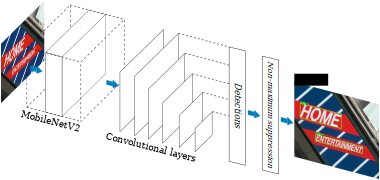
\includegraphics[width=\columnwidth]{ICIP_frankenstein/figs/proposed-method-overview.pdf}
%	\caption{Overview of the proposed method for text localization.}
%	\label{fig:architecture}
%\end{figure}
%\todo[inline]{Move this figure to the "Proposed Method" Section}

% %
% \begin{figure}[!t]
% 	\centering
% 	\includegraphics[height=0.066\textheight]{figs/examples/img_22.jpg}
% %	\includegraphics[height=0.08\textheight]{figs/examples/img_42.jpg}
% %	\includegraphics[height=0.08\textheight]{figs/examples/img_108.jpg}
% 	\includegraphics[height=0.066\textheight]{figs/examples/img_126.jpg}
% 	\includegraphics[height=0.066\textheight]{figs/examples/img_134.jpg}
% 	\includegraphics[height=0.066\textheight]{figs/examples/img_175.jpg}
% 	\caption{Example of challenge scene texts.}
% 	\label{fig:dataset-examples}
% \end{figure}
% %

Among the several approaches for localizing text in images, deep-learning-based techniques are the most promising strategies to reach high detection accuracy. \etal{He}~\cite{He2016TIP}, for example, presented a novel technique for scene text detection by proposing a Convolutional Neural Network (CNN) architecture that focuses on extracting text-related regions and specific characteristics of a text. The authors introduced a deep multi-task learning mechanism to train the Text-CNN efficiently, in which each level of the supervised information (text/non-text label, character label, and character mask) is formulated as a learning task. Besides, the authors proposed a pre-processing method, which extends the widely used Maximally Stable Extremal Regions (MSERs)~\cite{Matas2004IVC} by enhancing the local contrast between text and background regions. %The authors reported significant improvements in terms of recall and precision rates, in comparison with methods designed with traditional machine learning techniques for characterizing and learning high level information~\cite{Minetto2014CVIU}. 
Although the proposed CNN presented a reasonable efficiency in detecting candidate regions, with a processing time of about $0.5$ seconds per image, the pre-processing step requires about $4.1$ seconds per image, which may prevent a real-time detection. 

Another venue that may render outstanding results in terms of effectiveness consists of combining different deep learning architectures to benefit from complementary information to make a better decision. In this vein, \etal{Zhang}~\cite{Zhang2016CVPR} introduced an approach based on two Fully Convolutional Network (FCN) architectures for predicting a salient map of text regions in a holistic manner (named as \textit{Text-Block FCN}), and also for predicting the centroid of each character. The main idea of this approach consists of detecting text line blocks, which are more stable in comparison with character regions. Similarly, \etal{Tang} also proposed an ensemble of three modified VGG-16 networks~\cite{Tang2017TIP}: the first extracts candidate text regions (CTR); % of the scene image;  
the second network refines the coarse CTR detected by the first model, segmenting them into text; and finally, the refined CTR are served to a classification network to filter non-text regions and obtain the final text regions. The CTR extractor network is a modified VGG-16 that, in the training process, receives the edges of the text as supervisory information in the first blocks of convolutional layers and the segmented text regions in the last blocks. %Undoubtedly, 
Both strategies present several issues in terms of computational efficiency that could make their use unfeasible in restrictive computing scenarios.% (e.g., mobile devices).

Towards having a truthfully single-stage text detection, \etal{Liao}~\cite{Liao2018TIP} proposed an end-to-end solution named TextBoxes++, which handles arbitrary orientation of word bounding boxes, whose architecture inherits from the VGG-16 architecture. Similarly to TextBoxes++, \etal{Zhu} proposed a deep learning approach~\cite{Zhu2018TITS} also based on the VGG-16 architecture, but for detecting text-based traffic sign. Both techniques presented outstanding detection rates, but they rely on the use of VGG-16 architecture, which could be considered inadequate for restrictive computing scenarios due to its model size with about $138$ millions of parameters~\cite{Howard2017CoRR}, and floating-point operations per second (FLOPS) that reach about $15.3$ billion~\cite{HeCVPR2016}. In contrast, lighter CNN architectures, such as MobileNet~\cite{Howard2017CoRR}, present a very competitive alternative for this scenario, with a model size of $4.2$ millions of parameters and the FLOPS of $569$ million, for instance.

In light of these remarks, we propose a novel method for text localization considering efficiency and effectiveness trade-offs. Our approach, named MobText, combines two light architectures that were originally proposed for object detection -- MobileNetV2~\cite{Sandler2018CVPR} and SSD~\cite{Liu2016ECCV} -- and adapts them to our problem. The main contributions of this work are: 

\begin{itemize}
    \item (i) the proposal of an effective method for text localization task in scene images, which presented better or competitive results when compared with state-of-the-art methods at a low computational cost in terms of model size and processing time; 
    \item (ii) a comparative study, in the context of text localization, comprising widely used CNN architectures recently proposed for object detection;
    \item (iii) state-of-the-art results on the ICDAR'11 dataset, with F-Measure of $96.09\%$, and competitive results on ICDAR'13 with F-Measure of $73.58\%$; and
    \item (iv) proposal of an evaluation tool to support the assessment of text localization and recognition methods. %\todo[inline]{Provide contribution and adapt introduction to tool description}
\end{itemize}
%; and (iii) a study the most promising deep learning techniques for text recognition task?.

In summary, we addressed the following research questions:
\begin{itemize}
    \item Would a general-purpose object detection network, trained for the text detection task, achieve competitive results, in comparison with state-of-the-art methods?
   % \todo[inline]{Suggestion: Can an object detection network, trained for the text detection task, achieve competitive results, in comparison with state-of-the-art methods?}
    \item Would a mobile-oriented CNN architecture maintain a competitive performance on text detection while being light enough to be executed on devices with restricted computing power and built-in memory capacity?
    %\todo[inline]{Suggestion: Can a mobile-oriented CNN architecture maintain a competitive performance on text detection while being light enough to be executed on devices with restricted computing power and built-in memory capacity?}
    
    \item How to devise a generic evaluation tool to support the assessment of text localization and recognition methods?
\end{itemize}


%\etal{Gupta}~\cite{Gupta2016CVPR} proposed a new method for generating synthetic data for the text spotting problem, by blending synthetic text in natural images in order to have a scene text-like dataset, as illustrated in Figure~\ref{fig:Gupta2016CVPR-pipeline.png}. The authors also proposed a new FCN architecture for text/non-text detection. The SynthText dataset consists of synthetic text-scene images produced by a generation engine that localize the best location in a given image (e.g., contiguous regions) by using segmentation and geometry estimation algorithms and render a synthetic text in the found regions taking into account the local color and texture information to produce realistic scene-text images. The FCN network proposed by the authors based on \etal{Long}~\cite{Long2015CVPR} and \etal{Redmon}~\cite{Redmon2016CVPR} works. According to the authors, the improvements made in the YOLO architecture~\cite{Long2015CVPR} was crucial to achieve good results, in terms of accuracy, at a lower computation cost. The effectiveness of the proposed method was confirmed on ICDAR'11 and ICDAR'13 datasets, whose results were superior to works proposed in~\cite{Wang2012ICPR,Jaderberg2016IJCV,Neumann2012CVPR,Zhang2015CVPR}.

The remaining of this dissertation is organized as follows. Chapter~\ref{chap:related-work} introduces basic concepts related to the text detection problem, along with a brief background of technologies and techniques employed in this dissertation. Chapter~\ref{chap:proposed-method} presents MobText, the proposed method for text detection, besides the datasets, evaluation metrics, and protocols used to validate our approach, in comparison with baselines and their usage in real-world usage scenarios involving the use of mobile devices. This chapter also presents and discusses experimental results. %A description of the experiments made on a mobile, restrictive computing environment is provided in Chapter~\ref{chap:mobile-results}.
Chapter~\ref{chap:tool} describes the developed tool to support the evaluation of text localization and recognition methods.
Chapter~\ref{chap:conclusions} provides our conclusions over the results of our research and points out possible future work. 





In this chapter, a description of the proposed method is provided. Figure~\ref{fig:architecture} illustrates the overall framework of our approach for text localization, which uses MobileNetV2 as feature extractor and then SSD as multiple text bonding boxes detector. We detail the CNN architectures used, and then explain the learning mechanism used for finding a proper CNN model to the problem. Finally, we present and discuss performed experiments aiming to validate the proposed approach.

\begin{figure}[!ht]
	\centering
	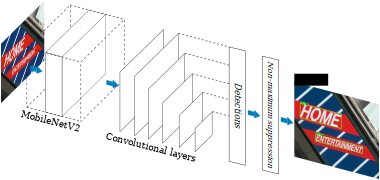
\includegraphics[width=\columnwidth]{ICIP_frankenstein/figs/proposed-method-overview.pdf}
	\caption{Overview of the Proposed Method for Text Localization.}
	\label{fig:architecture}
\end{figure}

\section{Characterization of Text Regions with MobilenetV2}

The MobilenetV2 is a new CNN specifically designed for restricted computing environments that includes two main mechanisms for decreasing the memory footprints and number of operations while keeping the effectiveness of its precursor architecture, the Mobilenet~\cite{Sandler2018CVPR}. Such mechanisms are the linear bottlenecks and the inverted residuals. Besides the depthwise separable convolution operations, which significantly reduce the FLOPS of a neural network, this new version of Mobilenet presents the linear bottleneck mechanism to reduce the number of parameters and keep the accuracy of the network by capturing a low-dimensional subspace (embedded in a manifold formed by a set of activation tensors). The authors claim that non-linearity reduces the capacity of bottleneck features to capture the most representative information. Thus, they decided to use a linear bottleneck, removing the ReLU activation.

The principles that guided the design of the inverted residual layers implemented on MobilenetV2 is that feature maps of the network are able to be encoded in low-dimensional subspaces, and non-linear activation causes some loss of information, notwithstanding their capability to increase representational complexity~\cite{Sandler2018CVPR}.

\begin{figure}[!ht]
	\centering
	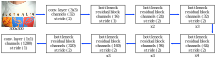
\includegraphics[width=\columnwidth]{ICIP_frankenstein/figs/feature-extraction-v1.pdf}
	\caption{MobilenetV2 architecture used in this work and its parameters. More details on the bottleneck residual block can be found in~\cite{Sandler2018CVPR}.}
	\label{fig:feature-extraction}
\end{figure}

Fig.~\ref{fig:feature-extraction} shows the MobilenetV2 architecture used to characterize text candidate regions. The \textit{bottleneck residual block} implements the optimization mechanisms aforementioned considering the convolutional operations with a kernel of size $3 \times 3$. The first bottleneck block uses an expansion factor of $1$, while the remaining blocks use an expansion factor of $6$, as suggested by \etal{Sandler}~\cite{Sandler2018CVPR}.

\section{Detecting Multiple Instances of Text via SSD}

The localization of text regions in scene images is challenging due to inherent variability of texts, such as size, color, font style, and distortions. 
The text localization should handle multiple scales and bounding boxes with varying aspect ratios. Although several authors consider the image pyramid for performing multi-scale detection, it is quite costly, which may be impractical for a restrictive computing scenario. Thus, we use the Single Shot detector~(SSD) framework~\cite{Liu2016ECCV}, a state-of-the-art method for object detection. The SSD approach includes a multiscale mechanism that allows the identification of text regions in multiple scales on a single inference. Specifically, in the framework, the authors adopt a top-down fusion strategy to build new features with strong semantics while keeping fine details. Text detections are performed based on multiple new constructed features respectively during a single forward pass. All detection results from each layer are refined by means of a non-maximum suppression (NMS) process~\cite{Neubeck2006ICPR}.

\section{Learning}

The main decisions we took in the learning phase of our network are:

\begin{itemize}

\item  {\bf Objective function:}
Similar to \etal{Liu}~\cite{Liu2016ECCV}, we use a multi-task loss function to learn the bounding boxes locations and text/non-text predictions (Equation~\ref{eq:loss}). Specifically, $x_{ij}$ indicates a match ($x_{ij} = 1$) or non-match ($x_{ij} = 0$) between $i$-th default bounding boxes, $j$-th ground-truth bounding boxes, $N$ is the number of matches, $c$ is the ground truth class of the $x_{ij}$ box and the $\alpha$ parameter is used as a multiplier of $\mathcal{L}_{loc}$ to weight the localization loss ($\mathcal{L}_{loc}$) and the confidence loss ($\mathcal{L}_{conf}$). The used loss function can be defined as:
%
\begin{equation}
    L(x,c,l,g) = \frac{1}{N} (\mathcal{L}_{conf}(x,c) + \alpha \mathcal{L}_{loc}(x, l, g))
    \label{eq:loss}
\end{equation}

We adopted the smooth L1 function for $\mathcal{L}_{loc}$ between the predicted box ($l$) and the ground truth box ($g$), and a sigmoid function for $\mathcal{L}_{conf}$. In addition, we set $\alpha=1$ in order to have the localization and confidence components with equal importance.

%\paragraph*{Hard example mining:}
\item {\bf Hard example mining:}
The hard example miner is a mechanism used to prevent imbalances between negative and positive examples during the training phase. On the search for text during the training, we usually have several non-text bounding boxes and few text bounding boxes. To mitigate the training with imbalanced data, we sort the negative bounding boxes according to their confidence, selecting the negative samples with higher confidence value, considering a ratio proportion of 3:1 with the positive samples.

\end{itemize}



%\subsubsection{Linear Bottlenecks}
%
%Beside of depthwise separable convolutions operations, this new version of MobilenetV2 presented the linear bottlenecks in the convolutional blocks aiming reducing the number of parameters of a neural network and capturing the low-dimensional subspace under the supposition that such low-dimensional subspace is embedded in manifold formed by a set of activation tensors. Although the authors did not show a mathematical demonstration that corroborate with this hypothesis, empirical evidences that the use of linear layers is important to prevent non-linearity added from  destroying information. Experiments conducted by the authors shows that non-linear bottlenecks, built with rectified linear units, can decrease the performance significantly in comparison with linear bottlenecks. In other words, the non-linearity can reduce the capacity of bottleneck features in capturing the most representative information.
%
%
%\subsubsection{Inverted residuals bottlenecks} 
%
%For mobile applications and other restrictive computing scenarios, the utilization of computational resources such as memory is crucial since high memory consuming is directly related to battery consumption, besides of provide, in some cases, a negative user experience. To understand how the inverted residual bottlenecks can help in using memory efficiently, we firstly need to understand how the memory-efficient inference works. Basically, a standard implementation builds a directed acyclic compute hyper-graph, in which the nodes represent the tensors and edges represent the operations, and computation (edges) should be scheduled in order to minimize the total number of tensors (nodes).
%


%The SSD-MobilenetV2 model, as described in~\cite{Sandler2018CVPR} was used as a text detector candidate model -- illustrated in Figure~\ref{fig:ssdmobilenet}. The SSDLite is a  mobile-friendly variant of the regular SSD, where the regular convolution layers are replaced by separable convolutions in SSD prediction layers. SSDLite dramatically reduces both parameter count (from 14.8M parameters to 2.1M) and computational cost (1.25B MAdds to 0.25B MAdds) compared to standard SSD. In this model, a Mobilenet V2 is used as a feature extractor for the SSDLite. 
%The MobilenetV2 is a neural network architecture that is designed for mobile and resource-constrained environments, retaining the accuracy of the much bigger and costly models.


\section{Experimental Protocol}
\label{sec:experiments-results}

This section presents the datasets,
metrics, 
and protocols used for evaluating the proposed method.

\subsection{Datasets}
We evaluated the proposed methods in two datasets widely used for evaluating text localization methods, the ICDAR'11 and ICDAR'13. We also used the SynthText dataset to help
training our network due to the small size of the ICDAR's datasets.

\begin{itemize}
    \item {\bf SynthText:} This dataset comprises $858,750$ synthesized text images, which were generated by blending rendered words with natural images~\cite{Gupta2016CVPR}. The synthetic engine proposed by the authors automatically choose the location, in a target image, and transforms a word by using an algorithm that selects contiguous regions based on local color and texture cues. Next, the words were rendered using a randomly selected font,
transformed according to the local surface orientation, and 
finally blended into the scene using the Poisson image editing approach~\cite{Perez2003ToG}.

\item{\bf ICDAR'11:} The ICDAR'11 dataset~\cite{Karatzas2011ICDAR} was introduced in \textit{ICDAR 2011 Robust Reading Competition -- ``Reading Text in Born-Digital Images (Web and Email)''}. 
It is an extension of the dataset used for the text locating competitions of ICDAR 2003~\cite{Lucas2003ICDAR} and ICDAR 2005~\cite{Lucas2005ICDAR}, and contains $551$ images, which were divided into two subsets, 
$410$ images for training and $141$ for test.
The images of this dataset have texts digitally created on them, such as headers, logos, captions, among others. The annotations were built in terms of rectangle word bounding boxes and contains $5,003$ words.

%\paragraph*{ICDAR'13:} 
\item{\bf ICDAR'13:}
This dataset was introduced in \textit{ICDAR 2013 -- ``Focused Scene Text challenge''} and has $462$ images divided into two subsets, training and testing sets, which contains $229$ and $233$ images, respectively~\cite{Karatzas2013ICDAR}. The images in this dataset are born-digital or scene text (captured under a wide variety, such as blur, varying distance to camera, font style and sizes, color, texture, etc). All the text lines are horizontal or near horizontal. The annotations were built in terms of rectangles word bounding boxes and comprise $1,943$ words.

\end{itemize}

\subsection{Evaluation Metrics}

We evaluated the methods in terms of effectiveness and efficiency, according to the metrics described as follow:

\begin{itemize}
\item{\bf  Effectiveness:} We evaluated the effectiveness of the methods in terms of recall, precision, and f-measure. %Here, we consider a correct detection (true positive) if the overlap between the ground-truth annotation and detected bounding box, which is measured by computing the intersection over union, is greater than $50\%$ (similar to standard practice in object recognition~\cite{Everingham2015}). Otherwise, the detected bounding box is considered an incorrect detection (false positive).

\begin{itemize}

      \item \textbf{Intersection over Union (IoU)} is used as protocol to measure the accuracy level between the text detected bounding boxes and the text ground-truth bounding boxes. 
    A detected bounding boxes is considered a correct detection (true positive), if the overlap between the ground-truth annotation and detected bounding box, which is measured by computing the Intersection of Union (Equation~\ref{eq:iou}), is greater than $50\%$. Otherwise, the detected bounding box is considered an incorrect detection (false positive). This protocol was proposed by \etal{Everingham} in the context of the PASCAL VOC challenge~\cite{Everingham2010IJCV} in 2009. Nowadays, it is adopted in ICDAR competitions.
    \begin{equation}
    IoU = \frac{area(B_p \cap B_{gt})}{area(B_p \cup B_{gt})},
    \label{eq:iou}
    \end{equation}
    where $B_p \cap B_{gt}$ and  $B_p \cup B_{gt}$ stand, respectively, for the intersection and the union of the predicted ($B_p$) and ground truth ($B_{gt}$) bounding boxes.
    %
    \item  \textbf{Recall ($R$)} refers to the fraction of text regions correctly detected, given the set of all text regions labeled in the dataset:
    \begin{equation}
        R = \frac{\sum \textrm{true positive}}{\sum (\textrm{true positive + false negative})}
    \end{equation}
    %
    \item  \textbf{Precision ($P$)} refers to the fraction of text regions correctly detected, given all text regions detected by the text detector:
    \begin{equation}
        P = \frac{\sum \textrm{true positive}}{\sum (\textrm{true positive + false positive})}
    \end{equation}
    %
    \item \textbf{F-measure} combines $P$ and $R$, allowing the possibility of having one single effectiveness score to assess the overall quality of a detector. It is defined as:
    \begin{equation}
        \textrm{F-measure} = 2 \times \left( \frac{P \times R}{P + R} \right)
    \end{equation}
    %
  
\end{itemize}

%\todo[inline]{DEFINE THE METRICS!!!!!}

%\paragraph*{Efficiency:} 
\item {\bf Efficiency:} The efficiency aspects considered both the processing time and the disk usage (in MB). We used the Linux {\em time} command to measure the processing time, %since this tool can be applied to all evaluated methods, regardless the programming language.
while the disk usage considered the size of the learned models. %and excluding the disk usage regarding the source code and the possible libraries used by the methods (e.g., Tesseract (tessdata) tool).
All experiments were performed considering a Intel(R) Core(TM) i7-8700 CPU @ 3.20GHz with 12 cores, a Nvidia GTX 1080 TI GPU, and 64GB of RAM.
% \begin{itemize}
%     \item \textit{CPU}: Intel(R) Core(TM) i7-8700 CPU @ 3.20GH;
%     \item \textit{GPU}: Nvidia GTX 1080 ti 11GB and Nvidia GTX Titan X 12GB;
%     \item \textit{Memory RAM}: 62GB;
%     \item \textit{Operating system}: Ubuntu 16.04 LTS (Xenial Xerus).
% \end{itemize}
\end{itemize}

\subsection{Evaluation Protocols}
\label{sec:protocols}

Here, we describe the experimental protocols used for evaluating the proposed method. 

\subsubsection{Comparisons with Baselines}

The experiments were divided into three steps: training, fine-tuning, and test. For the training step, we used three subsets of the SynthText dataset. This dataset comprises of images with synthetic texts added in different backgrounds and we selected samples of the dataset considering $10$ ($9.25\%$), $20$ ($18.48\%$), and $30$ ($27.71\%$) images per background. The resulting subsets were again divided into train and validation, using $70\%$ for training and $30\%$ for validation. Using these collections, we trained a model with random initialization parameters until we found no significant variance in the loss function. For the fine-tuning step, we took the model trained in SynthText and continued this training using ICDAR'11 or ICDAR'13 training subsets, stopping when we found no significant variance in the loss function. Finally, for the test step, we evaluated each fine-tuned model in the test subset of ICDAR'11 or ICDAR'13.

\begin{itemize}
\item {\bf Experimental setup}

We conducted the training of the proposed method considering a single-scale input, and therefore, all input images were resized to $300 \times 300$ pixels. The training phase was performed using a batch size of $24$ and we used the RMSprop optimizer~\cite{Tieleman2012} with a learning rate of $4 \times 10^3$. We also use the regularization L2-norm, with a $\lambda=4 \times 10^5$, to prevent possible over-fitting. We conducted the training until the network converge.



\item{\bf Baselines}


This section provides an overview of the chosen methods for comparison purpose. For a fair comparison, we selected recent approaches specifically designed for a fast detection, including SqueezeDet and YOLOv3. We also use state-of-the-art methods for text localization as baselines.

\begin{itemize}
%\paragraph*{TextBoxes:} 
\item{\bf TextBoxes:} This method consists of a Fully Convolutional Network (FCN) adapted for text detection and recognition~\cite{Liao2017AAAI}. This network uses the VGG-16 network as feature extractor followed by multiple output layers (text-boxes layers), similar to SSD network. At the end, the Non-maximum suppression (NMS) process is applied to the aggregated outputs of all text-box layers. The authors also adopt an extra NMS for multi-scale inputs on the task of text localization.

\item{\bf TextBoxes++:} Liao et al.~\cite{Liao2018TIP} proposed an end-to-end solution able to predict arbitrary orientation word bounding boxes. This architecture is a Fully Convolutional Neural Network (FCN) that detects arbitrary-oriented text. This architecture is inherited from the  popular VGG-16  architecture used for the ImageNet competition. First, the last two FCN layers of VGG16 are converted into convolutional layers (conv6 and conv7). Next, other eight convolution layers divided into four stages (conv8 and conv11) with  different  resolutions  by  max-pooling  are  appended  after conv7. In the following, multiple output layers (text boxes layers) are inserted after the last and intermediate convolutional layers to predict text presence and bounding boxes. Finally, a non-maximum suppression (NMS) process is applied to the aggregated outputs of all text-box layers.

\item {\bf Single-Shot Text Detector (SSTD):} \etal{He}~\cite{He2017ICCV} designed a natural scene text detector that directly outputs word-level bounding boxes without post-processing, except for a simple NMS. The detector can be decomposed into three parts: a convolutional component, a text-specific component, and a box prediction component. The convolutional and box prediction components are inherited from the SSD detector~\cite{Liu2016ECCV} and the authors proposed a text-specific component which consists of a text attention module and a hierarchical inception module.

\item {\bf SqueezeDet:} This network was proposed to detect objects for the autonomous driving problem, which requires a real-time detection~\cite{Wu2017CVPRW}. The SqueezeDet contains a single-stage detection 
% pipeline, which comprises essentially three components: a FCN, a Convolutional layer, and a filtering stage to remove redundant bounding boxes. The FCN is responsible for generating the feature map, while % for the input images. Next, these feature maps are used to feed 
% the convolutional layer %, which 
% is responsible for detecting, localizing, and classifying objects at the same time. The non-maximum suppression (NMS) is also applied to remove the overlapped bounding boxes.
pipeline, which comprises three components: (i) a FCN responsible for generating the feature map for the input images; (ii)  a convolutional layer responsible for detecting, localizing, and classifying objects at the same time; and (iii) the non-maximum suppression (NMS) method, which is applied to remove the overlapped bounding boxes.

\item {\bf YOLOv3:} This is a convolutional network originally proposed for the object detection problem~\cite{Redmon2018CoRR}. Similarly to SSD network, the YOLOv3 predicts bounding boxes and class probabilities, at the same time. The bounding boxes are predicted using dimension clusters as anchor boxes and predicts an objectness score for each bounding box using logistic regression.

\end{itemize}

\end{itemize}

\subsubsection{Experiments on Mobile-Oriented Environment}

This section provides a description of experiments performed on a device with restricted computing capacity. %After a description of the  mobile device technical specifications, the experimental protocol is defined alongside with the data used to evaluate the solution.

To emulate the use of our proposed solution on real-world usage scenarios and to evaluate the performance on a real constrained computing, an Android application was developed and executed. The developed Android application (APP) utilizes TensorFlow~\cite{tensorflow}'s Android API so it can load and execute the same model used for inference in our previous evaluations. 
The chosen portable device for the implementation and execution of our test was a \textit{Xiaomi Redmi Note 5} smartphone, running Android OS version 9 on a \textit{Qualcomm Snapdragon 636} chipset, comprehending a quad-core 1.8Ghz processor alongside a quad-core 1.6Ghz processor and 4 Gb of RAM.

Two sets of experiments where conducted with the goal of assessing the embedded system: 
\begin{enumerate}
    \item Evaluation of the processing time of the proposed approach when running on a mobile device. Experiments considered the detection of images belonging to the ICDAR'11 and ICDAR'13 datasets; and
    \item Evaluation on a real-world mobile-based usage scenarios.
\end{enumerate}

To ensure that the model executed on the mobile device has the same quantitative effectiveness that the one executed on a non-restrictive computing scenario, the same experiments used to evaluate the proposal on the non-restrictive device were executed on the mobile device, conserving datasets and evaluation metric configurations.

The proposed solution was also evaluated in real-world usage scenarios. Given the portability of the embedded APP, the proposed approach was evaluated in detection scenarios involving several images depicting texts in scenes captured using the portable device. To evaluate the efficiency of the proposed method considering a restricted computing environment, we collected $250$ images containing text and non-text elements, captured directly from the built-in camera of the mobile device.



\label{chap:conclusions}

 \nobibliography*

How to perform efficient and effective text detection in scene images in restrictive computing environments? 
To address this research problem, we presented a new method based on the combination of two light architectures, MobileNetV2 and Single Shot Detector~(SSD), which yielded better or comparable effectiveness performance when compared with state-of-the-art baselines despite having a low processing time and small model size, being suitable for a restrictive computing environment.

This work resulted on a published conference paper~\cite{decker}:
\begin{itemize}
    \item \textbf{\bibentry{decker}}.
\end{itemize}

Also, this work contributed to other publications~\cite{joselito-paper,manuel,jhonny}. Appendix~\ref{appendix:A} comprehends a copyright disclaimer for partial use of indexed articles on dissertationsor thesis.


As contributions and answers to our research questions, we have that: 

\begin{itemize}
    \item \textbf{Would an object detection network, trained for the text detection task, achieve competitive results, in comparison with state-of-the-art methods?}
    
    \textbf{Yes}. Compared with other object detection solutions, our method is the most promising one in all evaluation criteria, yielding state-of-the-art on ICDAR'11 dataset and competitive results in ICDAR'13, alongside very satisfactory results on images obtained from the wild. Our findings disagree with the discussion provided in~\cite{Ye2015PAMI}, as we demonstrated that adapting object detector networks for text detection is a promising research venue, besides the system still being sensitive to visual abnormalities such as reflections and deformations.
    
    \item \textbf{Would a mobile-oriented CNN architecture maintain a competitive performance on text detection while being light enough to be executed on devices with restricted computing power and built-in memory capacity?}
    
    \textbf{Yes.} Our method, when executed on a real application on a mobile, computational restrictive device, maintained the performance and had very promising processing time, showing itself suitable for being applied on a embedded system. 
    
    \item \textbf{How to devise a generic evaluation tool to support the assessment of text localization and recognition methods?}
    
     Two types of approaches were considered in the implementation of text detection and recognition approaches: methods that do not rely on deep learning strategies; and methods that take advantage of deep learning-based architectures. The prototype also includes post-processing components, which may be used to improve text detection results.
    
    
\end{itemize}

There is still a lot of work to be done with the scenario of text detection and recognition in devices with restricted computing power that can be a future work after our proposal, such as:

\begin{itemize}
    \item Improve the system to detect multi-oriented text, extending the capabilities of the proposal to multi-oriented text dataset such as ICDAR'15.
    
    \item Improve the architecture of the feature extractor network, aiming for a smaller processing time, consequently a smaller energy impact, and/or the extraction of better features, allowing to detect text on images with abnormalities.
    
    \item Extend the proposed approach for the detection of multi-language text. The goal is to efficiently recognize characters and sentences in languages different from the Latin-derived, such as Chinese, Japanese, Korean, Hindi and Arabic. 
    
    \item Create mobile-based applications that can benefit from the proposed lightweight architecture.
    
    \item Extend the evaluation tool to encapsulate different evaluation protocols, including, among others, datasets, and performance evaluation metrics. 
    
    \item Extend the evaluation tool to simulate scenarios commonly found when handling restrictive computing devices. This infrastructure may contribute, for example, to speed up the development of new text localization and recognition methods customized for specific constrained hardware configurations.
    
    \item Extend the evaluation tool to include a graphical user interface, which would support the selection of text detection and recognition methods.
    
    \item Extend the evaluation tool to support the creation of new applications based on implemented methods. One starting point would be the creation of an application that exploits contextual information provided by text recognition methods.
    
    \item Extend the evaluation tool to support fusion strategies of the different methods for text spotting and recognition.
    
\end{itemize}



\vfill\pagebreak
% References should be produced using the bibtex program from suitable
% BiBTeX files (here: strings, refs, manuals). The IEEEbib.bst bibliography
% style file from IEEE produces unsorted bibliography list.
% -------------------------------------------------------------------------
\bibliographystyle{IEEEbib}
\bibliography{bib/IEEEabrv,bib/others-abbrev,bib/maestro-samsung,bib/maestro-samsung-idar-ijdar}

\end{document}
